\documentclass[Conference]{IEEEtran}
\usepackage[utf8]{inputenc}
\usepackage{cite} % cite{label}
\usepackage{amsmath} % bmatrix
\usepackage[pdftex]{graphicx}
\usepackage{adjustbox}

\usepackage{algorithm}% For algorithm table
\usepackage{algpseudocode}% For algorithm table


\title{Estimating 3D Structure from Motion using\\
the Normalized Eight Point Algorithm\\
and LUP Decomposition\\}
\begin{document}

\author{
\IEEEauthorblockN{Alexander Koumis\\}
\IEEEauthorblockA{Computer Engineering Department\\
San Jose State University\\
me@alexander.computer}}

\maketitle

\begin{abstract}
This paper examines the Eight-point algorithm, which computes a Fundamental matrix from a pair of feature sets extracted from two images of the same scene. The RANSAC scheme is then used to remove outliers by performing the algorithm repeatedly on the point sets, removing those which fall beneath a set threshold.
\end{abstract}

\section{Introduction}
Recently published work regarding 3D reconstruction ~\cite{Hartley2004} presents new market opportunities in the areas of surveillance, autonomous vehicle networks, augmented reality, and more. SfM (Structure from Motion), or obtaining a 3D representation of a physical object based on an image set of said objects, provides a wealth of information for such aforementioned fields, giving robotic systems a better understanding of the world around them. Photogrammetric methods of capturing 3D representations of scenes and objects are also compellingly cheaper than their laser-based (LIDAR) alternatives.
In this work, the \textit{Normalized eight-point algorithm} is examined as a means of extracting the Fundamental matrix, used to estimate 3D coordinates based on 2D parameters.

\section{Background and Objectives}
Modern photogrammetry-influenced SfM pipelines have several options for computing estimated 3D world points from a pair of 2D features, extracted from two images. Most SfM algorithms involve computation of $F$, the Fundamental Matrix, introduced by Q. T. Luong~\cite{AICPub329:1992}, a parametrized way to describe the 3D relationship between a pair of feature matches, satisfying homogeneous equation~\eqref{eq:fundamental}~\cite{Hartley2004}. $x$ and $x'$ are determined by extracting keypoints and/or descriptors from two images, using any number of algorithms, such as SIFT~\cite{Bay:2008:SRF:1370312.1370556}, SURF~\cite{Bay:2008:SRF:1370312.1370556},  using sets extracted from 2D images, wthe column-extended 2D feature coordinates (equation \eqref{eq:points}) with all $z$ values in $x$ and $x'$ set to 1).

\begin{center}
    \begin{equation}\label{eq:fundamental}
        {x}'^TFx = 0
    \end{equation}
\end{center}


\begin{align}\label{eq:points}
    x = 
    \begin{bmatrix}
        x_1 & y_1 & z_1\\ 
        x_2 & y_2 & z_2\\ 
        \vdots&\vdots&\vdots\\ 
        x_n&y_n&z_n\\
    \end{bmatrix}
    &&
    x` =
    \begin{bmatrix}
        x`_1 & y`_1 & z`_1\\ 
        x`_2 & y`_2 & z`_2\\ 
        \vdots & \vdots & \vdots\\ 
        x`_n&y`_n&z`_n\\
    \end{bmatrix}
\end{align}


\subsection{Eight point algorithm}
The eight point algorithm, introduced by Longuet-Higgens in 1987 ~\cite{Longuet-Higgins:1987:CAR:33517.33523}, assumes the left hand side of equation~\eqref{eq:fundamental} as a singular value, equals to zero with 9 unknowns, which can therefore be solved with 8 linearly independent vectors. Rearranging equation~\eqref{eq:fundamental} by multiplying both sides by ${x}^-1$ allows the problem to be expressed as equation~\eqref{eq:Af}, where $A$ is defined as the $n x 9$ cross product of each match pair in $x$ and $x'$.

As the measurements are typically noisy, the solution must be calculated as a least squares minimization, where $||f||=1$, achievable by setting $F_{33}$ to 1. With $z_i$  and $z'_i$ also both equals to 1, $A$ becomes a square 8x8 matrix (see equation~\eqref{eq:expanded8Pt}, accurate to scale (projective accuracy rather than Euclidean), allowing $F$ to be solved using one of several linear solvers. LU decomposition with partial row pivoting is explored in this paper.

\begin{equation}\label{eq:Af}Af=0\end{equation}

\begin{align}\label{eq:fullFundamental}
    \resizebox{0.5\textwidth}{!}{
        $\begin{bmatrix}
            x_1x_1' & y_1x_1' & z_1x_1' & x_1y_1' & y_1y_1' & z_1y_1' & x_1z_1' & y_1z_1' & z_1z_1'\\
            \vdots&\vdots&\vdots&\vdots&\vdots&\vdots&\vdots&\vdots&\vdots\\
            x_nx_n' & y_nx_n' & z_nx_n' & x_ny_n' & y_ny_n' & z_ny_n' & x_nz_n' & y_nz_n' & z_nz_n'\\
        \end{bmatrix}
        \begin{bmatrix}
            F_{11}\\F_{12}\\F_{13}\\F_{21}\\F_{22}\\F_{23}\\F_{31}\\F_{32}\\F_{33}
        \end{bmatrix}$
        =0
    }
\end{align}

\begin{align}\label{eq:expanded8Pt}
    \resizebox{0.5\textwidth}{!}{
        $\begin{bmatrix}
            x_1x_1' & y_1x_1' & x_1' & x_1y_1' & y_1y_1' & y_1' & x_1 & y_1\\
            x_2x_2' & y_2x_2' & x_2' & x_2y_2' & y_2y_2' & y_2' & x_2 & y_2\\
            x_3x_3' & y_3x_3' & x_3' & x_3y_3' & y_3y_3' & y_3' & x_3 & y_3\\
            x_4x_4' & y_4x_4' & x_4' & x_4y_4' & y_4y_4' & y_4' & x_4 & y_4\\
            x_5x_5' & y_5x_5' & x_5' & x_5y_5' & y_5y_5' & y_5' & x_5 & y_5\\
            x_6x_6' & y_6x_6' & x_6' & x_6y_6' & y_6y_6' & y_6' & x_6 & y_6\\
            x_7x_7' & y_7x_7' & x_7' & x_7y_7' & y_7y_7' & y_7' & x_7 & y_7\\
            x_8x_8' & y_8x_8' & x_8' & x_8y_8' & y_8y_8' & y_8' & x_8 & y_8
        \end{bmatrix}
        \begin{bmatrix}
            F_{11}\\F_{12}\\F_{13}\\F_{21}\\F_{22}\\F_{23}\\F_{31}\\F_{32}
        \end{bmatrix}$
        =0
    }
\end{align}

\subsection{Normalized eight point algorithm}

The traditional eight point algorithm has been criticized for producing inaccurate results, given the aforementioned presence of inevitably noisy measurements.  Hartley’s 1997 ~\cite{Hartley:1997:DEA:262631.262634} defense of the eight point algorithm states the algorithm is fundamentally sound in theory, and simply needs normalization of its input parameters to produce more robust results. The errors, he suggests, stem from the fact that the arbitrary $1$ chosen for the third dimension of $x$ and $x`$ are not normalized with respects to the first and second dimensions.
His solution comes in form of the \textit{Normalized eight point algorithm}, described in figure ~\ref{algorithm}. The algorithm first computes the centroid for both sets of points, or the normalized average of the values in each dimension:

\begin{align}\label{eq:centroid}
    c =\begin{bmatrix}
        \frac{\sum_{i}^{8}x_i}{8\sqrt{2}} & \frac{\sum_{i}^{8}y_i}{8\sqrt{2}} & \frac{\sum_{i}^{8}z_i}{8\sqrt{2}}
    \end{bmatrix}
&&
    c' =\begin{bmatrix}
        \frac{\sum_{i}^{8}x'_i}{8\sqrt{2}} & \frac{\sum_{i}^{8}y'_i}{8\sqrt{2}} & \frac{\sum_{i}^{8}z'_i}{8\sqrt{2}}
    \end{bmatrix}
\end{align}

The average distance from each point sets' centroid is calculated, by finding the average magnitude of difference between each point's coordinate and the centroid:

\begin{align}\label{eq:avgDistance}
    dist = \frac{
        \sum_{i}^{8}
        \sqrt{x_i^{2}+y_i^{2}+z_i^{2}}
    }{8}
&&
    dist' = \frac{
        \sum_{i}^{8}
        \sqrt{x`_i^{2}+y`_i^{2}+z`_i^{2}}
    }{8}
\end{align}

The points are then scaled by the inverse of the average distance, which are then plugged into equation ~\eqref{eq:expanded8Pt}:

\begin{align}\label{eq:scale}
    scale = \frac{1}{dist}
&&
    scale' = \frac{1}{dist'}
\end{align}

\begin{align}\label{eq:pointsScaled}
    x = \begin{bmatrix}
        \frac{x_1}{scale} & \frac{y_1}{scale} & \frac{z_1}{scale}\\[0.3em]
        \frac{x_2}{scale} & \frac{y_2}{scale} & \frac{z_2}{scale}\\[0.3em]
        \vdots & \vdots & \vdots\\ 
        \frac{x_n}{scale} & \frac{y_n}{scale} & \frac{z_n}{scale}\\[0.3em]
    \end{bmatrix}
&&
    x' =
    \begin{bmatrix}
        \frac{x'_1}{scale'} & \frac{y'_1}{scale'} & \frac{z'_1}{scale'}\\[0.3em] 
        \frac{x'_2}{scale'} & \frac{y'_2}{scale'} & \frac{z'_2}{scale'}\\[0.3em]
        \vdots & \vdots & \vdots\\ 
        \frac{x'_n}{scale'} & \frac{y'_n}{scale'} & \frac{z'_n}{scale'}\\[0.3em]
    \end{bmatrix}
\end{align}
\\
The scaled points are then plugged into equation ~\eqref{eq:expanded8Pt}


$F$ is de-normalized using, producing more stable values than would have been gathered sans normalization.



\subsection{Triangulation}
After $F$ has been calculated, 3D world point estimated can be made computing $P$ and $P`$, the estimated projection matrices of each cameras, satisfying equations \eqref{eq:xPX_1} and \eqref{eq:xPX_2}. $P$ is taken to be the canonical projection, with $P`$ describing the rotation and translation of the second image projection relative to the first. \textbf{e`} is defined as the \textit{epipole} of the second image, or the position of the projection of the first camera's centroid on the second image (see figure \ref{fig:homography}), and is computed as the left nullspace of $F$~\eqref{eq:F_left_nullspace}.

\begin{equation}\label{eq:xPX_1}\end{equation}
\begin{equation}\label{eq:xPX_2}\end{equation}
\begin{equation}\label{eq:P}\end{equation}
\begin{equation}\label{eq:P_prime}\end{equation}
\begin{equation}\label{eq:F_left_nullspace}\end{equation}


The \textit{RANSAC} (Random sample consensus) scheme is used to determine an optimal set of 8 matches to finally use in equation \ref{eq:fullFundamental}. It's operation is outlined in figure \ref{algo:RANSAC}. 8 matches from the image pair are repeatedly chosen with the \textit{normalized 8 point algorithm} used to compute $F$. For a predefined number of iterations, 8 random point matches are selected and used to fill up 


\begin{figure}
\begin{center}
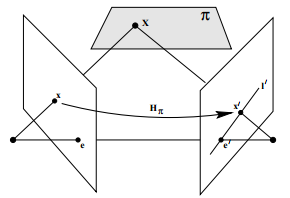
\includegraphics[scale=0.6]{images/homography.png}
\caption{Estimating 3D feature coordinate from 2D features~\cite{Hartley2004}}
\label{fig:homography}
\end{center}
\end{figure}

\begin{algorithm*}
    \caption{RANSAC outlier removal}
    \begin{algorithmic}[1]
        \Procedure{RANSAC Outlier Removal}{$x, x', maxIterations, threshold$}
        \While{$count\not=maxIterations$}
            \State $x[8][3]\gets get8random(x)$
            \State $x'[8][3]\gets get8random(x')$
            \State $F\gets estimateFlinear(x, x')$
            \State $removeOutliers(F)$
            \State $count\gets count+1$
        \EndWhile\label{RANSACOutliers}
        \State \textbf{return} $F$
        \EndProcedure
    \end{algorithmic}
\label{algo:RANSAC}
\end{algorithm*}


\section{Findings and Analysis}
Wow this stuff is sweet.

\section{Conclusion and Recommendations}
The conclusion goes here.

\bibliography{sfm}{}
\bibliographystyle{IEEEtran}

\end{document}

